\section{Two grammars for the top of the board}
\label{sec:systems}

Every published solution is a combination of two components: \emph{generative members},
which supply the structural signal of Section~\ref{sec:generator}, and a \emph{stack}, which
supplies variance reduction. The mixture explains the shape of Table~\ref{tab:board}: the
winner used both; the 4th place used only generative members and no public predictions; the
7th, 11th and 16th put a generative family on top of a large public stack; and the 25th,
28th and 29th ran stacks of discriminative members alone, landing at 0.9624.

\begin{figure}[t]
\centering
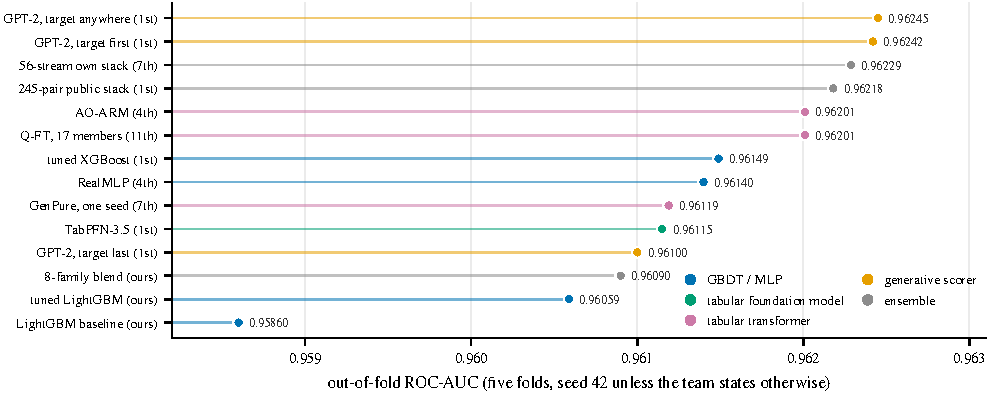
\includegraphics[width=\linewidth]{figures/fig_ladder.pdf}
\caption{Single-model \auc{} on the shared folds, as reported by the teams. Bars are drawn
from 0.9582 to the value; colour marks the model family. The row marked ``ours'' is this
repository's eight-family blend, i.e.\ what a conventional pipeline reaches. Every
generative scorer except the discriminative reading sits above it, and the best one is a
124M GPT-2.}
\label{fig:ladder}
\end{figure}

\subsection{Generative members: four implementations of one idea}

\paragraph{GPT-2 with the target first (1st).}
A stock GPT-2 small is fine-tuned for 60 epochs on the original survey and 8 epochs on the
competition rows, with the columns in random order; at prediction time 30 random orders are
combined with a log-sum-exp. Formatting follows the original file exactly (integer age,
one-decimal delays, \texttt{None} for missing), the GPT-2 tokenizer is used rather than a
digit-wise one, and cases are left as in the source. Ten such members (small, medium and
large backbones, target first/anywhere, plus a GPT-Neo variant) carry about 80\% of the
final stack's output~\citep{kaggle_first}.

\paragraph{AO-ARM (4th).}
A from-scratch encoder replaces GPT-2: every column value becomes a learned embedding
(column embedding plus value embedding, with a separate vocabulary per column), the model
is an any-order autoregressive transformer, and classification is the averaged
log-likelihood difference over 32 random column orders, one model per fold. Twenty-one
AO-ARM streams carry about 70\% of the net standardised coefficients of a 189-stream
logistic stack, and one recipe alone scores 0.96258 on private~\citep{kaggle_fourth}.

\paragraph{GenPure (7th).}
Twenty-one tokens per row from a vocabulary built on train and test features only; numeric
values seen fewer than three times are merged into coarse bins. A 6-layer, 256-wide,
8-head causal transformer models $P(x,y)$ with a new random column order per batch; the
score is the log-mean-exp of the Bayes log-odds over eight fixed orders. Unlabelled rows
(train-test and held-out folds) contribute a feature-likelihood term with weight 0.5, and
each fold gets Platt scaling on a 10\% inner holdout, which also picks the epoch. Two
choices mattered: pure generative training (adding a BCE term on the log-odds lowered OOF
from 0.95960 to 0.95907) and training longer (12 $\to$ 36 epochs, +0.0016 per seed,
early stopping off)~\citep{kaggle_seventh}.

\paragraph{Q-FT and Q-FT v2 (shared by 1st, 9th, 11th).}
Q-FT feeds 22 learned vectors per row (21 features plus a CLS) into a frozen Qwen3-0.6B
decoder through LoRA, with column embeddings initialised from the word vectors of the column
names, per-value lookup tables that include one entry per flight-distance ``route'', and
periodic numeric embeddings~\citep{kaggle_qft}. Version~2 replaces the decoder with a
bidirectional ModernBERT encoder, sets every \texttt{position\_ids} to zero so the row is
read as a set, adds side features and two summary tokens, and pretrains on replaced-token
detection: 149M parameters, $6.5$ minutes per fold on one A100, OOF 0.960798 against Q-FT's
0.959795~\citep{kaggle_qft2,warner2024modernbert}. The 11th-place team's 17 Q-FT members
moved their stack from 0.96213 to 0.96241~\citep{kaggle_eleventh}.

\subsection{The stack: a shared pool and a regularised linear head}

The second component is boring on purpose. Every team converted probabilities to logits,
standardised them with statistics from the training part of the meta-fold, and fitted an
$L_2$ logistic regression; the differences are the pool and the shrinkage.

\begin{itemize}
  \item \textbf{Pool.} Public OOF/test pairs on the same five folds accumulated from 119
        columns on 6 October to 245 by 20 October and 284--531 by the deadline; teams
        deduplicated at a logit correlation of 0.999 and verified each file's row order and
        fold assignment. Figure~\ref{fig:pools} shows who used how much.
  \item \textbf{Shrinkage.} $C=0.3$ for a 56-column own-only stack, $C=0.003$ for 299--312
        columns, $C=0.01$ for 364. The 29th-place team reports that re-tuning $C$ from 0.1
        to 0.01 when their pool grew from 199 to 364 members was worth \dlt{0.3} --- more
        than any single new member they added later~\citep{kaggle_twentyninth}.
  \item \textbf{Non-linear heads are optional.} The 25th-place team averaged
        $0.8\,z(\text{LR})+0.2\,z(\text{LightGBM})$ over 299 columns; the 28th-place team
        tried an $L_1$ logistic (470 inputs, 173--192 non-zero coefficients per fold) and a
        CatBoost on logits initialised from a logistic margin. Both landed within
        \dlt{0.2} of plain $L_2$ logistic~\citep{kaggle_twentyfifth,kaggle_twentyeighth}.
\end{itemize}

\begin{figure}[t]
\centering
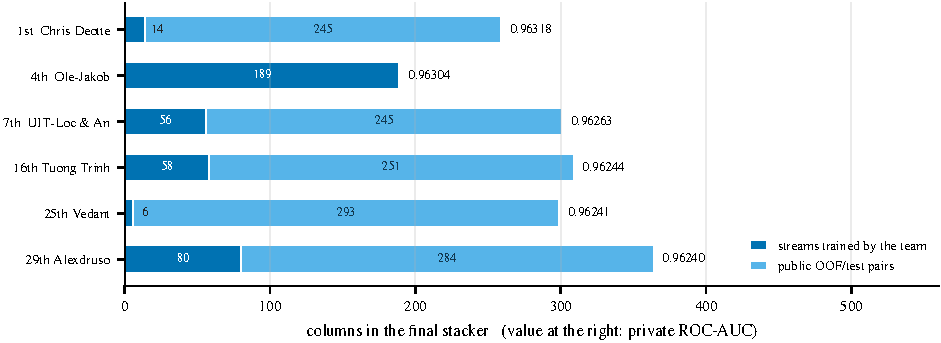
\includegraphics[width=\linewidth]{figures/fig_pools.pdf}
\caption{Composition of the final stacker for the six teams that state exact counts.
Blue: streams the team trained; light blue: public OOF/test pairs. Two routes reach the
top: 189 own streams and no public predictions (4th), or a handful of own generative
members plus the shared pool (1st). The number at the right of each bar is the private
\auc.}
\label{fig:pools}
\end{figure}

Table~\ref{tab:systems} summarises the published pipelines. The rightmost column is the
honest one: how much of each team's final score is attributable to a component that other
teams could not have copied from the public pool.

\begin{table}[t]
\centering
\small
\caption{Published solutions at a glance. ``Own'' and ``public'' count streams entering the
final stacker; ``CV'' and ``private'' are the team's own reported numbers.}
\label{tab:systems}
\begin{tabular}{p{2.05cm}p{1.8cm}p{7.95cm}rr}
\toprule
Team & own / public & ingredients, and what was new & CV & private\\
\midrule
1st Deotte & 14 / 245
  & GPT-2 $\times$10, nine TFMs, GBDTs. Target-first scoring on a GPT-2 fine-tuned on the
    original survey; ten such members carry most of the output
  & 0.96290 & 0.96318\\
4th Ole-Jakob & 189 / 0
  & AO-ARM $\times$21 plus XGBoost, RealMLP, CatBoost, TabPFN. Any-order transformer scored
    by likelihood; no public predictions used
  & 0.96279 & 0.96304\\
5th Mohsen & many / many
  & Not disclosed. Stack of own and shared OOF; CV-only selection in the final week
  & 0.96270 & 0.96292\\
7th UIT & 56 / 245
  & GenPure $\times$16 plus RealMLP, TabPFN, CatBoost, set transformers. Bagged generative
    transformer with Bayes scoring; two submission slots
  & 0.96247 & 0.96263\\
9th Cremer & $\approx$20 / 4
  & A pretrained transformer plus LightGBM, kNN and MLP. Masked-token and replaced-token
    pretraining on train$+$test
  & 0.96213 & 0.96259\\
11th Feng & 300+ / 3
  & XGBoost, LightGBM, CatBoost, RealMLP and 17 Q-FT members; 300-column $L_2$ logistic
  & 0.96241 & 0.96254\\
16th Trinh & 58 / 251
  & 42 feature-view GBDTs, TabPFN, a GPT-2 row classifier. GReaT surrogate likelihood ratios
    and a residual LightGBM on the offsets
  & --- & 0.96244\\
25th Singhal & 6 / 293
  & Six own members plus 293 community columns; 0.999 deduplication, LR/LightGBM 80/20
  & 0.96222 & 0.96241\\
29th Alexdruso & 80 / 284
  & LightGBM, RealMLP, kNN, EBM on feature views. Route-id target encoding; $C=0.01$ on 364
    columns
  & 0.96227 & 0.96240\\
\bottomrule
\end{tabular}
\end{table}

